\documentclass[12pt,a4paper]{scrartcl}

\usepackage[utf8]{inputenc}
\usepackage{graphicx}
\usepackage[ampersand]{easylist}
\usepackage[printonlyused]{acronym}

\usepackage{url}
%\urldef{\urlTcpdump}{\url}{http://www.tcpdump.org/}
\urldef{\urlARSupport}{\url}{http://api.rubyonrails.org/classes/ActiveRecord/Migration.html#class-ActiveRecord::Migration-label-Database+support}

\usepackage{hyperref}
\hypersetup{colorlinks=false,pdfborder={0 0 0}}

\usepackage{biblatex}
\ExecuteBibliographyOptions{hyperref=true,language=ngerman,backref=true}
\addbibresource{bibliography.bib}

% Shorten the usage of german quotation marks.
\newcommand{\gq}[1]{
	\glqq #1\grqq
}

% Inline comment.
\newcommand{\comment}[2]{#2}
\newcommand{\todo}[2]{#2}

% Vertical space after paragraph.
\newcommand{\s}{\vspace{0.5em}}

% Little table for most important software info.
\newcommand{\infotable}[4]{
	\begin{tabular}{p{2.5cm}l}
		Website: & \url{#1} \\
		Language: & #2 \\
		Last commit: & #3 \\
		Commits: & #4 \\
	\end{tabular}
	\s
}

% Emphasize a criterion.
\newcommand{\crit}[2]{\textbf{#1} (#2)}

% Aliases for yes and no in comparison overview table.
\newcommand{\y}{\checkmark}
\newcommand{\n}{$\times$}

% Easy reference to section name and page.
\newcommand{\textref}[1]{"\nameref{#1}" on page \pageref{#1}}

% Palatino
\renewcommand*\rmdefault{ppl}
%\renewcommand{\baselinestretch}{1.125}
\renewcommand{\baselinestretch}{1.1875}

% Times
%\usepackage{times}

% Iwona
%\renewcommand*\rmdefault{iwona}



\begin{document}

	\title{Møil: A web-based administration tool for mail servers backed by relational databases}
	\author{Henning Müller $<$\href{mailto:henning@orgizm.net}{henning@orgizm.net}$>$}
	\date{}

	\maketitle


	\section*{Abstract}
		This document compares existing administration user interface solutions
		for mail servers backed by relational databases and introduces yet
		another one, which is called \emph{Møil} and is written in Ruby
		utilizing the \ac{Rails}\footnote{\url{http://rubyonrails.org}}
		framework. It brings the handy possibility of managing the database
		schema with migrations, a lot of beautiful, responsive \acs{CRUD} and
		some other nice features (see page \pageref{sec:moeil:features}). The
		code is available from
		GitHub\footnote{\url{https://github.com/nning/moeil}} licensed under
		AGPLv3 \cite{agpl}.

	\section*{Introduction}
		% Reasons for database-backing

		For mail system setups (meaning one or more servers running Mail
		Submission, Delivery and Transfer Agent software and providing a
		Message Store for users \cite{mail-architecture}), storing data about
		which domains and E-Mail addresses the system is responsible for
		(further called meta data) in relational databases (as opposed to plain
		files for example) is beneficial for several reasons.

		%	Horizontal scalability

		In bigger setups, it offers the possibility for scaling to more than
		one node (horizontal scalability) to cope with high mail and user
		loads: Several servers handling incoming mail or users reading their
		mail act as readers on one or more database servers. The performance of
		the frequent lookups of domains, mailboxes and aliases (forwardings)
		for receiving mail or user logins can be increased. (The actual
		accommodation of E-Mails -- another big problem with horizontal scaling
		-- can not be considered here.)

		%	API (e.g. for accounting)

		\acp{DBMS} for relational databases usually provide a query interface
		with the \ac{SQL} \cite{sql} for editing the data sets. It is widely
		supported by programming languages and equally widely spoken among
		programmers, which makes it valuable for integration of several
		services dealing with this mail system meta data. For example this can
		be used to integrate accounting solutions for charging purposes into
		mail systems.

		%	Structural clarity for administrators

		Another reason for the usage of relational databases as mail system
		meta data storage is the increased structural clarity for
		administrators. In a typical \acs{SMTP} \cite{smtp} server setup
		(without a relational database), the relevant data for domains,
		mailboxes and aliases is distributed to several files. The existence of
		a domain is stated independently of the existence of a mailbox of the
		same domain or the password of this mailbox. The data is not
		interconnected; a mailbox address is usually not checked against the
		list of domains for consistency. For bigger mail system setups, this
		meta data configuration inevitably gets unmaintainable.

	\section*{Evaluation of existing software}
		% Overview and inspiration

		Although an extensive evaluation of the existing administration user
		interfaces did not happen before implementing a custom solution, some
		of the programs were still sighted and some of the following criteria
		was still considered. This more systematical and detailed analysis
		shall gain an overview and provide inspiration for the development of
		\emph{Møil}.

		\subsection*{Criteria}
			Not only for the development of \emph{Møil}, some of the criteria
			arose from shortcomings of \emph{postfix.admin} (see page
			\pageref{sec:contestants:postfix.admin}), which is a quite widely
			deployed solution. The criteria will be classified into five
			categories (Data model, features, security \& robustness, user
			interface and miscellaneous) and numbered for easier reference.

			\subsubsection*{Data model (1)}
				From a database engineering perspective, it is in general
				favourable to design a database with a \crit{normalized
				relational database schema}{1.1} \cite{dbnorm}. For a query to
				check the existence of a mailbox for example, a JOIN or nested
				query would be necessary, which has a very small performance
				impact. However, the schema normalization prevents data
				redundancies and inconsistencies. \emph{postfix.admin} does not
				have a normalized schema, so any solution which has one can not
				be \crit{compatible to \emph{postfix.admin}}{1.2}. A
				compatibility could be useful, if there is a big database
				already administered with \emph{postfix.admin}, which shall be
				migrated to another tool. Another possibility for this is an
				\crit{import of \emph{postfix.admin} data}{1.3}. When it comes
				to updates to the administration interface, \crit{means to
				handle database schema updates}{1.4} ease the update process
				(and therefore increase the probability of the actual
				conduction of an update). Last but not least, \crit{database
				independence}{1.5} allows a free choice of the \ac{DBMS} and
				integration with other software.

			\subsubsection*{Features (2)}
				There are features, without which a mail server admistration
				user interface would not work at all and yet I list them,
				because it is more about analyzing, how these are implemented.
				The \crit{basic domain, mailbox and alias management}{2.1} is
				one of them. The \crit{password changing ability for
				users}{2.2} is a feature, which is also quite basic and the
				first one legitimating letting users access the administration
				frontend. Some solutions also integrate into popular
				self-hosted web mailer software for password changing. When
				users are allowed to access the administration frontend,
				\crit{access control}{2.3} or authorization is needed to
				selectively restrict the access to resources. It could also be
				possible to delegate administrative access on domains or
				resources in general to certain users.
				\s

				More mature utilities also bring useful non-basic features as
				an \crit{audit trail}{2.4.1} for example, which can be used to
				log any changes to the database with time and transacting
				account. It is also possible, the audit trail provides an undo
				functionality. In some environments users demand \crit{vacation
				mailing}{2.4.2} to automatically answer any incoming mail with
				a pre-defined text when they are vacant. Some solutions serve
				users with the possibility to activate or deactivate it and
				edit the pre-defined text. Automatic answers can also be solved
				more generic with \crit{Sieve}{2.4.3} \cite{sieve}, which is a
				server-side mail filter interface. The protocol for users to
				edit the server-side filters is called \emph{ManageSieve}
				\cite{managesieve}. Another common demand of users of a mail
				system is a \crit{spam frontend}{2.4.4} to review mails, which
				got quarantined by spam or virus checking software. (Although in
				my personal experience this false negative classification does
				occure almost never with a setup common in the Open Source
				world consisting of \emph{amavisd-new}, \emph{spamassassin} and
				\emph{clamav}.)

			\subsubsection*{Security \& robustness (3)}

			\subsubsection*{User interface (4)}

			\subsubsection*{Miscellaneous (5)}

		\subsection*{The contestants}
			\subsubsection*{modoboa}
				\infotable{http://modoboa.org}{Python}

				\emph{modoboa} seems the most mature of the compared tools. It
				uses the Python Django framework and therefore includes
				facilities like schema migrations.

			\label{sec:contestants:postfix.admin}
			\subsubsection*{postfix.admin}
				\infotable{http://postfixadmin.sourceforge.net}{PHP}

%				As said, \emph{postfix.admin} seems to be a (negative) example
%				not only for \emph{Møil}. Many solutions aim to overcome its
%				shortcomings. \emph{postfix.admin} uses a non-normalized
%				\cite{dbnorm} database schema, which could spare a JOIN in some
%				database queries but is very prone to inconsistencies. There
%				are no means of handling database schema updates; the schema is
%				imported via a \ac{SQL} file on the initial installation. Also
%				it creates an alias entry for every mailbox (even when the mail
%				is not forwarded). This may have a cause, but is messy anyway.

			\subsubsection*{PostVis Admin}
				\infotable{http://postvisadmin.sourceforge.net}{PHP}

			\subsubsection*{ratuus}
				\infotable{http://www.ratuus.org}{PHP}

			\subsubsection*{VBox.Adm}
				\infotable{http://www.vboxadm.net}{Perl}

			\subsubsection*{ViMbAdmin}
				\infotable{http://www.vimbadmin.net}{PHP}

	\section*{Møil}
		The development of \emph{Møil} has been begun in May, 2013 as an Open
		Source project licensed under the terms of the AGPL, Version 3
		\cite{agpl}.

		% Rails
		
		It is written in Ruby\footnote{\url{https://www.ruby-lang.org}}
		utilizing the popular \ac{Rails} web framework, which has some features
		that emphasize it against other frameworks or web development
		approaches. It promotes the development by \acs{REST} \cite{rest}
		criteria, supports test driven development and implements many
		well-known software engineering design patterns and methods of agile
		software development as Active Record, \ac{CoC}, \ac{DRY} and \ac{MVC}.
		Additionally, the \ac{Rails} community is quite vivid and there is an
		huge ecosystem of extensions for many recurrent problems.
		\s

		% Causes for a new solution
		%	Data model, migrations
		%	CLI
		%	Password hash generation for compatibility to older solution

		That fact alone would maybe suffice as an argument for the development
		for yet another tool but was not as important as some other ideas.
		\emph{Møil} began as a replacement for the database schema shipped with
		\emph{postfix.admin} in a private mail system of mine. The schema
		was intended to be reimplemented normalized \cite{dbnorm} and with
		a possibility of being updated through schema
		migrations\footnote{\url{http://en.wikipedia.org/wiki/Schema_migration}}).
		Also, the \ac{Rails} project was intended to provide the basis for
		command line utilities to import the existent data and to perform basic
		administration tasks on domains, mailboxes and aliases. As there has
		been only the schema in use, not the whole \emph{postfix.admin} web
		frontend, there was an extra solution to generate password hashes and
		send them to an administrative contact in place. A replacement for this
		extra tool at first was the only function of the web interface part of
		\emph{Møil}. The migration opportunity was also used to change the
		password hashing algorithm from unsalted \texttt{md5} to
		\texttt{sha512-crypt}, which is substantially more secure
		\cite{missing}. (\texttt{bcrypt} was considered but unfortunately
		rejected, because it is not supported by \texttt{glibc} included in
		Debian Linux 7.)

		\todo{Sources for algorithms and their comparisons}

		%	Other features?

		\label{sec:moeil:features}
		\subsection*{Features}
			At the time of writing of this document, \emph{Møil} comes with the
			below-mentioned features.

			\begin{description}
				\item[\rm Managing domains, aliases and mailboxes]\ \\
					\todo

				\item[\rm Tested with postfix and dovecot]\ \\
					There are some produtive installations of \emph{Møil} in
					connection with postfix and dovecot but it could possibly
					also be used with other mailing software which provides the
					opportunity to configure the \ac{SQL} statements used to
					request necessary meta data.
				
				\item[\rm Database agnostic]\ \\
					\emph{Møil} is tested mostly on SQLite3 and PostgreSQL but
					also occasionally on MySQL (or MariaDB respectively). In
					general, it should be supported on any database supported
					by \emph{Active Record}, which currently are (at least)
					MySQL, PostgreSQL, SQLite, SQL Server, Sybase, and all
					supported Oracle databases except
					DB2\footnote{\urlARSupport}.

				\item[\rm Track database schema with rails migrations]\ \\
					Through \emph{Active Record} and \ac{Rails} migrations,
					\emph{Møil} has a robust solution for database change
					management. This also makes individual changes to the
					database schema easily maintainable.

				\item[\rm Permissions and Roles]\ \\
					The abilities to manage domains and/or subordinate resources
					like mailboxes and aliases can be configured fine grained
					in order to delegate administrative tasks.

				\item[\rm Responsive user interface]\ \\
					\emph{Møil} adapts to the environment, it is needed in. The
					web user interface is responsive and therefore supports
					both classic desktop view ports and mobile devices like
					phones or tablets. For friends of the command line, some
					commands to manage the most important resources are
					provided, too.

				\item[\rm Audit log]\ \\
					Any change to resources is logged with time and acting
					mailbox to support the collaboration of several different
					administrative users and to implement the possibility of
					reverting changes.

				\item[\rm Search]\ \\
					A search for any resources is provided, which is optionally
					based on \ac{SQL} or elasticsearch for really huge
					databases (if installed and configured to be used).
			\end{description}

		\subsection*{Architecture}
			% Modules

		\subsection*{Data model}
			% Data model
			%	Structure / ERD

			The application model is put into graphs in the following image. It
			shows the model classes and their relations among each other. (The
			graph is generated, so unfortunately (for now) the actual attributes
			saving a relation are missing.)

			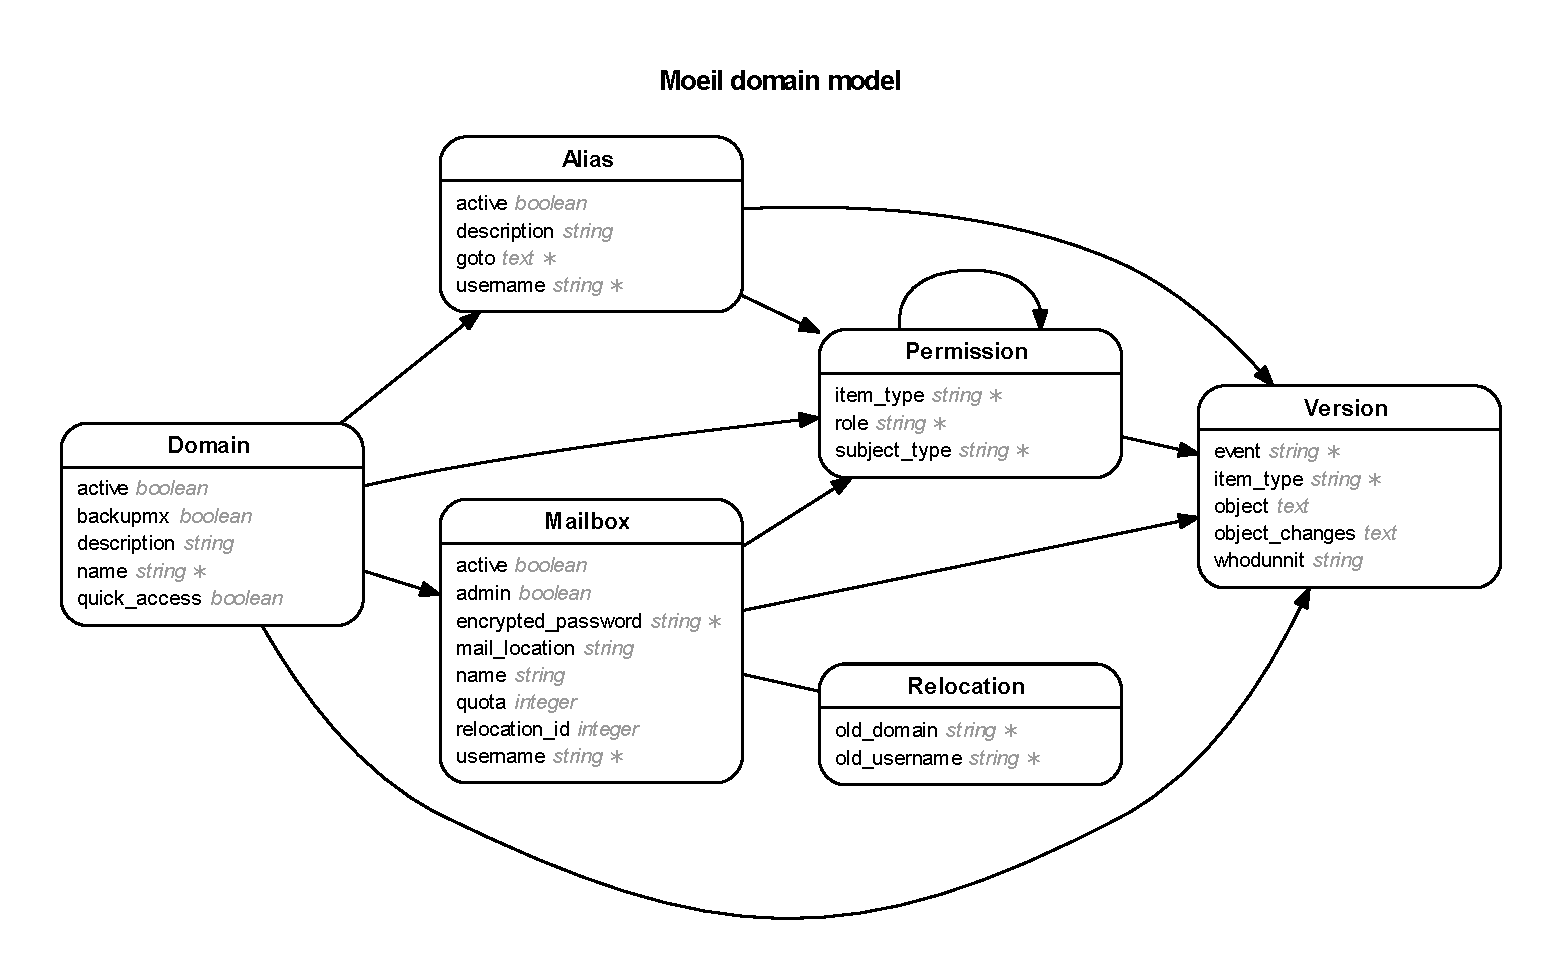
\includegraphics[width=\textwidth]{images/erd.pdf}

			The model classes will be examined individually in the following
			subsections.
			\s

			In this chapter, whenever a resource type is mentioned, which
			corresponds to an actual \ac{Rails} model class, it is written in a
			monospace font and -- as the class name -- capitalized, like
			\texttt{Mailbox}. Attributes of models are also in monospace font,
			but lowercase, as the \texttt{username} attribute of a
			\texttt{Mailbox} for example.

			\subsubsection*{Domains}

			\subsubsection*{Mailboxes}

			\subsubsection*{Aliases}

			\subsubsection*{Permissions}
				\texttt{Mailbox} records (or users) are also used for the login
				to \emph{Møil}. There are administrators and regular users.
				Administrators are allowed to edit any resources. Through a
				\texttt{Permission}, a \texttt{Mailbox} (the \texttt{subject})
				can be given access to \texttt{Domains} (the \texttt{item}).
				The rights on these \texttt{Domains} depend on the
				\texttt{role} of the user in this context. With an owner
				\texttt{role}, users can manage any aspect of the
				\texttt{Domains}. The editor \texttt{role} allows users to
				manage \texttt{Mailboxes} and \texttt{Aliases} of that.
				\texttt{Domain}. The \texttt{Permission} model is implemented
				polymorphic. Its \texttt{subject} and \texttt{item} attributes
				are not bound to \texttt{Mailboxes} and \texttt{Domains} (as in
				the current implementation). It is possible to extend the
				implementation easily to allow even more fine-grained
				permissions (for certain \texttt{Mailboxes} for example).

			\subsubsection*{Versions}
				As seen in the graph, \texttt{Domains}, \texttt{Mailboxes},
				\texttt{Aliases} and \texttt{Permissions} are versioned, which
				means that changes to resources of any of these types are
				tracked in the audit log and are revertable for administrators.
				On any change, a reference to the corresponding resource
				(\texttt{item\_id} and \texttt{item\_type}), the type of change
				(\texttt{event}), the transacting individual
				(\texttt{whodunnit}), the serialized \texttt{object} (only on
				deletions), the \texttt{object\_changes} (only on updates) and
				the point in time (\texttt{created\_at}) are saved.

			\subsubsection*{Relocations}
				The relocation model is in fact updated but actually not
				further used, currently. Whenever a \texttt{Domain} or
				\texttt{Mailbox} is renamed, it is necessary to move the
				corresponding folders in the file system of the Mail Store.
				These moves are represented as \texttt{Relocation} resources
				saving \texttt{old\_domain} and \texttt{old\_username} values,
				which can be read by a daemon (yet to be implemented) running
				on the actual Mail Store.

				\todo{Other solutions?}

			%	Migrations
			%	sha512-crypt

		\subsection*{Perspective}
			% Better CLI
			% Spam
			% Sieve

		\subsection*{Setup}
			% Relevant configs for postfix and dovecot
			% Setup of rails app
			% Links to README on GitHub

	\appendix

	\newpage
	\section*{Numbered index of criteria}
		\begin{easylist}
			& Data model
			&& Normalized schema
			&& \emph{postfix.admin} compatible
			&& \emph{postfix.admin} import
			&& Updatable (Migrations)
			&& Database independence

			& Features
			&& Basic domain, mailbox and alias management
			&& Password changing for users
			&& Access control
			&& Others
			&&& Audit trail
			&&& Vacation
			&&& Sieve
			&&& Spam frontend

			& Security \& robustness
			&& Password hashing
			&& Tests

			& User interface
			&& Responsiveness
			&&&	\ac{CLI} support
			&&& Mobile devices
			&& Usability

			& Miscellaneous
			&& Scalability
			&& Programming language
			&& Containability (e.g. independence of Message Store file system)
		\end{easylist}

	\newpage
\section*{Acronyms}
\begin{acronym}
	\acro{CLI} {Command line interface}
	\acro{CRUD}{Create, read, update and delete}
	\acro{DBMS}{Database Management System}
	\acro{SMTP}{Simple Mail Transfer Protocol}
	\acro{SQL} {Structured Query Language}
\end{acronym}


	\printbibliography

\end{document}
